
\section{Zusammenfassung}
\label{sec:zusammenfassung}

\todo[inline, color=green]{Jan}


\section{Einleitung}
\label{sec:einleitung}

\todo[inline, color=green]{Jan}


\subsection{Kontext/Hintergrund}


\subsection{Projekt Motivation}


\subsection{Problemstellung}


\subsection{Projektziele}


\subsection{Projektumfang}


\subsection{Übersicht über die Dokumentation}


\section{Methodik}
\label{sec:methodik}

\todo[inline, color=green]{Simon}


\subsection{Prinzipienschaltbild}
\label{subsec:prinzipienschaltbild}

Der prinzipielle Aufbau des Projekts wurde zuerst erstellt und in einem Blockdiagramm dargestellt, dass die verschiedenen Komponenten und deren Verbindungen veranschaulicht. Dieses Diagramm zeigt den Fluss des Zugangskontrollsystem von Authentifizierung und Temperaturmessung über das Schreiben in die Datenbank bis hin zur Ansteuerung der Drehkreuzes und der Lichtschranken.
\todo{Bildgröße am Ende anpassen}

\begin{figure}[h]
	\centering
	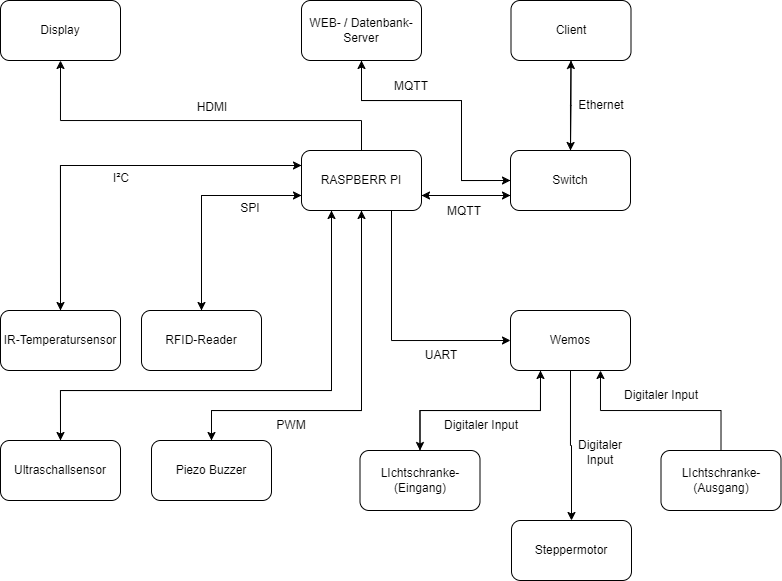
\includegraphics[width=0.4\linewidth]{figures/Prinzipienschaltbild.png}
	\caption[Prinzipienschaltbild]{Schematischer Aufbau des Projekts}\label{fig:prinzipienschaltbild}
\end{figure}


\subsection{Die Wahl der Hardware}
\label{subsec:die_wahl_der_hardware}

\subsubsection{Raspberry-Pi}

Der Raspberry Pi verfügt bereits über eine Vielzahl an Schnittstellen, die eine einfache Integration von Sensoren, Aktoren und weiteren Peripheriegeräten ermöglicht. Durch vorhandenes Wissen und umfangreiche Dokumentationen kann die Umsetzung der Anforderungen effizient erfolgen, ohne dass eine aufwendige Einarbeitung in neue Hardware notwendig ist. Zudem stellt der Raspberry Pi eine kostengünstige und vielseitige Plattform dar, die eine schnelle Entwicklung, Erprobung und iterative Optimierung technischer Lösungen unterstützt.

\subsubsection{Display}

Das Display wird verwendet, um dem Nutzer visuell relevante Informationen wie den aktuellen Status des Systems, Zugangsberechtigungen oder Fehlermeldungen bereitzustellen. Durch die grafische Darstellung kann der Benutzer schnell und intuitiv auf wichtige Systeminformationen zugreifen, was die Bedienfreundlichkeit und Effizienz des Systems erhöht. Das Display sorgt dafür, dass der Nutzer klare Informationen über das System erhält. Unter anderem mit Farben oder Symbolen wird angezeigt, ob der Zugang erlaubt oder verweigert wird. So bekommt der Nutzer direktes Feedback und Missverständnisse werden vermieden.

\subsubsection{RFID-Reader}

Der RFID-Reader wird im Zugangssystem zur Authentifizierung verwendet, indem er die individuellen Daten von RFID-Tags ausliest, die jedem Mitarbeiter zugeordnet sind. Jeder Tag enthält eine einzigartige ID, die mit einer gespeicherten Liste von Berechtigungen abgeglichen wird, um zu entscheiden, ob der Zugang gewährt oder verweigert wird. Diese personalisierte, berührungslose Authentifizierung bietet eine schnelle und sichere Möglichkeit, den Zugang für berechtigte Personen zu steuern.

\subsubsection{Infrarot-Temperatursensor}

Ein Infrarot-Temperatursensor misst schnell und kontaktlos die Körpertemperatur eines Mitarbeiters. Liegt die Temperatur über einem festgelegten Schwellenwert, wird der Mitarbeiter als potenziell krank eingestuft. Diese Methode ist hygienisch, schnell und verhindert die Verbreitung von Krankheiten im Arbeitsumfeld.

\subsubsection{Piezo-Buzzer}

Der Piezo-Buzzer wird verwendet, um dem Nutzer akustisches Feedback zu geben, indem er bei bestimmten Ereignissen wie dem erfolgreichen oder fehlgeschlagenen Zugang ein Signal abgibt. Durch die Erzeugung von Tönen oder Melodien kann der Benutzer sofort erkennen, ob eine Aktion erfolgreich war oder eine Fehlermeldung vorliegt. Der Buzzer sorgt für eine klare, hörbare Rückmeldung, die das visuelle Feedback des Systems ergänzt und so die Benutzererfahrung verbessert, indem er Missverständnisse verhindert und sofortige Reaktionen ermöglicht.

\subsubsection{Ultraschallsensor}

Der Ultraschallsensor erkennt die Annäherung eines Mitarbeiters und aktiviert automatisch das Display. So wird das System effizient und benutzerfreundlich ohne manuelles Eingreifen aktiviert.

\subsubsection{Wemos ESP32 D1 Mini}

Der Wemos D1 Mini ESP32 wurde aufgrund seiner kompakten Größe und ausreichenden GPIO-Pins für die Steuerung der Lichtschranken und des Steppermotors gewählt. Da er über UART an einen Raspberry Pi angeschlossen wird, ermöglicht der Wemos eine einfache und effiziente Kommunikation zwischen den Komponenten bei gleichzeitig platzsparender Bauweise.

\subsubsection{Lichtschranke}

Die Lichtschranke wird eingesetzt, um zu erkennen, wenn jemand versucht, durch das Drehkreuz zu gehen. Sobald der Infrarotstrahl unterbrochen wird, signalisiert die Lichtschranke dem System, dass sich eine Person im Drehkreuzbereich befindet, und löst daraufhin die entsprechende Aktion aus, wie zum Beispiel das Öffnen des Drehkreuzes. Diese Technologie ermöglicht eine präzise Erkennung der Passage und sorgt für eine automatische, kontaktlose Steuerung des Zugangs.

\subsubsection{Steppermotor}

Der Steppermotor wird verwendet, um ein Drehkreuz zu simulieren, indem er präzise Drehbewegungen ausführt. Durch die Steuerung des Motors kann das Drehkreuz geöffnet oder geschlossen werden, je nachdem, ob ein Mitarbeiter Zugang erhält. Diese Methode ermöglicht eine exakte und zuverlässige Steuerung der Drehmechanik, was für den reibungslosen Ablauf des Zugangssystems entscheidend ist.

\subsubsection{WEB-Datenbank-Server}

Ein Web- und Datenbankserver wird für die Steuerung, Überwachung und Speicherung des Zugangskontrollsystems genutzt. Er verwaltet Benutzerzugänge, speichert Transaktionsprotokolle und ermöglicht eine zentrale Überwachung und Verwaltung des Systems.

\subsubsection{Switch}

Für die Netzwerkkommunikation wird ein Switch eingesetzt, um die Verbindung zwischen den verschiedenen Geräten im System zu ermöglichen. Der Switch sorgt für eine effiziente und zuverlässige Datenübertragung, indem er die Geräte im Netzwerk miteinander verbindet und den Datenverkehr optimiert.

\subsubsection{Zusammenfassung}

Die ausgewählten Komponenten bieten eine effiziente und zuverlässige Lösung für das Zugangskontrollsystem. Sie ermöglichen eine benutzerfreundliche Interaktion, präzise Erfassung von Daten und Sicherheitsüberprüfungen. Ein zentraler Server verwaltet die Daten, während eine stabile Netzwerkverbindung die Kommunikation zwischen den Geräten sicherstellt. So wird eine zuverlässige Steuerung und Überwachung des Zugangsprozesses gewährleistet.


\subsection{Bestimmung der Messwerte}

Im Rahmen der Implementierung des Zugangskontrollsystems werden verschiedene Messwerte erfasst, um die Funktionalität des Systems sicherzustellen. Die Messwerte werden kontinuierlich überprüft und validiert, um die Genauigkeit und Zuverlässigkeit der Systeme zu gewährleisten.

\subsubsection{Bestimmung der Körpertemperatur}

Die Körpertemperatur wird durch einen Infrarot-Temperatursensor (MLX90614) gemessen, der die Umgebungstemperatur und die Temperatur des Mitarbeiters erfasst. Der Sensor arbeitet kontaktlos und liefert schnell Ergebnisse.

\vspace{1em}
\noindent Um die Validität der gemessenen Temperatur zu überprüfen, wird der Sensorwert mit den Messwerten eines Referenzthermometers verglichen. Bei größeren Abweichungen erfolgt eine Kalibrierung des Sensors, um genaue und zuverlässige Temperaturdaten zu gewährleisten. Diese Validierung stellt sicher, dass die Temperaturmessung präzise ist und eine korrekte Entscheidung darüber getroffen werden kann, ob ein Mitarbeiter als potenziell krank eingestuft wird.

\subsubsection{Bestimmung des Abstandes (Näherungssensor)}

Der Abstand wird durch einen Ultraschallsensor gemessen, der die Entfernung zum Objekt ermittelt. Der Sensor sendet Schallwellen aus und misst die Zeit, die benötigt wird, damit die Wellen zurückkehren. Diese Zeitdifferenz wird verwendet, um die Entfernung in Zentimetern zu berechnen.

\vspace{1em}
\noindent Die Messwerte des Ultraschallsensors wurden durch den Vergleich mit einer physischen Messung mit einem Meterstab validiert. Der ermittelte Wert des Sensors wurde mit den Werten des Meterstabs verglichen, um sicherzustellen, dass die Entfernungsmessung korrekt ist. Diese Methode gewährleistet eine präzise Erkennung der Annäherung eines Mitarbeiters an das System.


\section{Software und User Interface}
\label{sec:software_und_user_interface}

\todo[inline, color=green]{Leopold}


\subsection{Messsoftware}
\label{subsec:messsoftware}

Die Messsoftware dieses Projekts setzt sich aus mehreren Programmen zusammen.
Die genaue Funktionsweise und Interaktionen der einzelnen Programme miteinander werden nun im Folgenden erklärt.


\subsection{Datenbanksystem}
\label{subsec:datenbanksystem}


\subsubsection{Einführung}

Das Datenbanksystem (DBS) wurde ursprünglich mit SQLite3 implementiert, da es relativ einfach und intuitiv zu handhaben ist benutz haben wir eine SQL Row based Datenbank. Allerdings ergeben sich hierbei Probleme bei mehrfachen Zugriffen auf die Datenbank. Um diese Herausforderungen zu lösen, wurde auf ein Server-Client-Modell mit PostgreSQL umgestellt.


\subsubsection{Problemstellung bei SQLite3}

SQLite3 basiert auf Binärcode, was zu Problemen führen kann, wenn zwei Anwendungen gleichzeitig auf die gleiche Datenbank zugreifen. In diesem Szenario schreibt das Prozessprogramm (Python) die Messwerte in die Datenbank, während die GUI (Webapplikation) die Daten aus der Datenbank liest. Wenn das Prozessprogramm gerade Daten in die Datenbank schreibt, wird diese blockiert. Dadurch kann nicht gleichzeitig aus der Datenbank gelesen werden.


\subsubsection{Lösung: Umstellung auf PostgreSQL}

Um die gleichzeitige Nutzung durch mehrere Anwendungen zu ermöglichen, wurde auf PostgreSQL umgestellt. Als Open-Source-Datenbank bietet PostgreSQL folgende Vorteile:

\begin{itemize}
    \item Multi-User-Unterstützung: Mehrere Clients können gleichzeitig auf den zentralen Server zugreifen.
    \item Transaktionssicherheit: Durch den Einsatz von Transaktionen werden Schreib- und Lesevorgänge konsistent und sicher abgewickelt.
    \item Erweiterbarkeit: Zahlreiche Erweiterungen und Anpassungsmöglichkeiten machen PostgreSQL zu einer flexiblen Lösung.
    \item Netzwerkbasierter Zugriff: Das System kann als zentraler Datenbankserver in unterschiedlichen Umgebungen eingesetzt werden.
\end{itemize}

Aktuell läuft der PostgreSQL-Server auf einem Raspberry Pi. Eine zukünftige Weiterentwicklung sieht jedoch den Betrieb auf einem zentralen Server vor, wobei einzelne Komponenten wie die grafische Benutzeroberfläche (GUI) ebenfalls ausgelagert werden könnten.


\subsubsection{Schematischer Aufbau}
\label{subsubsec:schematischer_aufbau}

\begin{figure}[h]
	\centering
	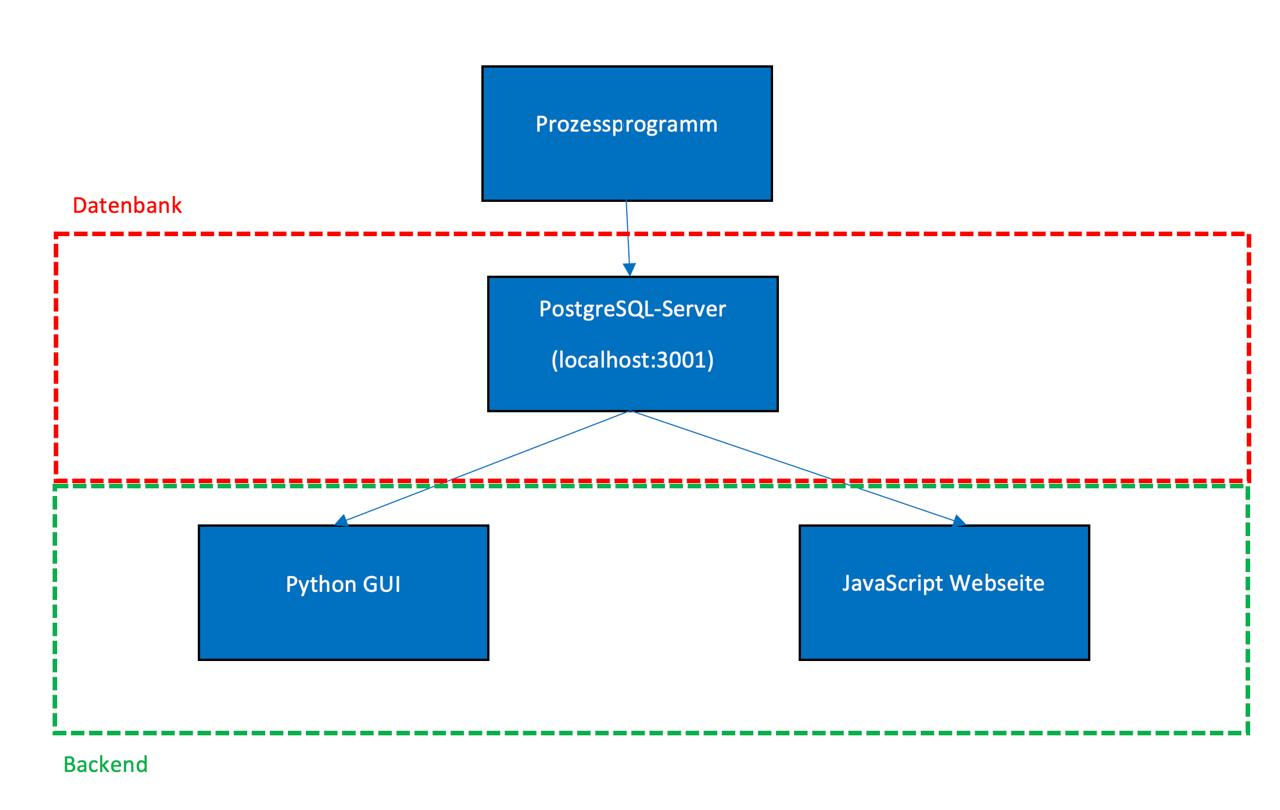
\includegraphics[width=0.4\linewidth]{figures/Schematischer Aufbau.jpeg}
	\caption[Schematischer Aufbau]{Schematischer Aufbau des Datenbanksystems}\label{fig:schematischer_aufbau}
\end{figure}
\todo{Bildgröße am Ende anpassen}


\subsubsection{Zusammenfassung}
\label{subsubsec:zusammenfassung}

Durch PostgreSQL wird ein robustes und flexibles Datenbanksystem geschaffen, das die Vorteile beider Technologien vereint. Das Frontend in Python erlaubt eine lokale Steuerung, während die Website als Verwaltungspunkt für einen Admin dient. Insgesamt lässt sich das System als lehr- und praxisnah bewerten.


\subsection{Technologien und Architektur}
\label{subsec:technologien_und_architektur}


Für die Umsetzung der Webanwendung haben wir uns für einen aktuellen Technologie-Stack entschieden, der uns viel Flexibilität und eine klare Struktur bietet:

\begin{itemize}
    \item \textbf{HTML5 \& CSS3:}\newline Die Grundstruktur der Anwendung basiert auf HTML5. Für das Styling nutzen wir CSS3 in Kombination mit Tailwind CSS, was uns ein responsives und ansprechendes Design ermöglicht.
    \item \textbf{JavaScript \& Chart.js:}\newline Dynamische Inhalte und interaktive Elemente werden mit JavaScript realisiert. Für die Darstellung von Diagrammen, etwa zur Visualisierung von Temperaturverteilungen oder Mitarbeiterrollen, setzen wir auf Chart.js.
    \item \textbf{RESTful API:}\newline Um eine reibungslose Kommunikation zwischen Frontend und Backend sicherzustellen, verwenden wir eine RESTful API, die im JSON-Format arbeitet. Über diese Schnittstelle werden Funktionen wie die Benutzerregistrierung, der Login, die Mitarbeiterverwaltung und diverse Datenbankabfragen abgewickelt.
    \item \textbf{Responsive Design:}\newline Dank moderner CSS-Frameworks und responsiven Layouts passt sich die Anwendung automatisch an verschiedene Geräte an – egal, ob auf dem Desktop oder auf mobilen Geräten.
\end{itemize}


\subsection{Benutzerinterface und Funktionalitäten}
\label{subsec:benutzerinterface_und_funktionalitäten}

Das Benutzerinterface ist in mehrere Bereiche unterteilt, um die Bedienung möglichst einfach zu gestalten. 

\begin{figure}[h]
	\centering
	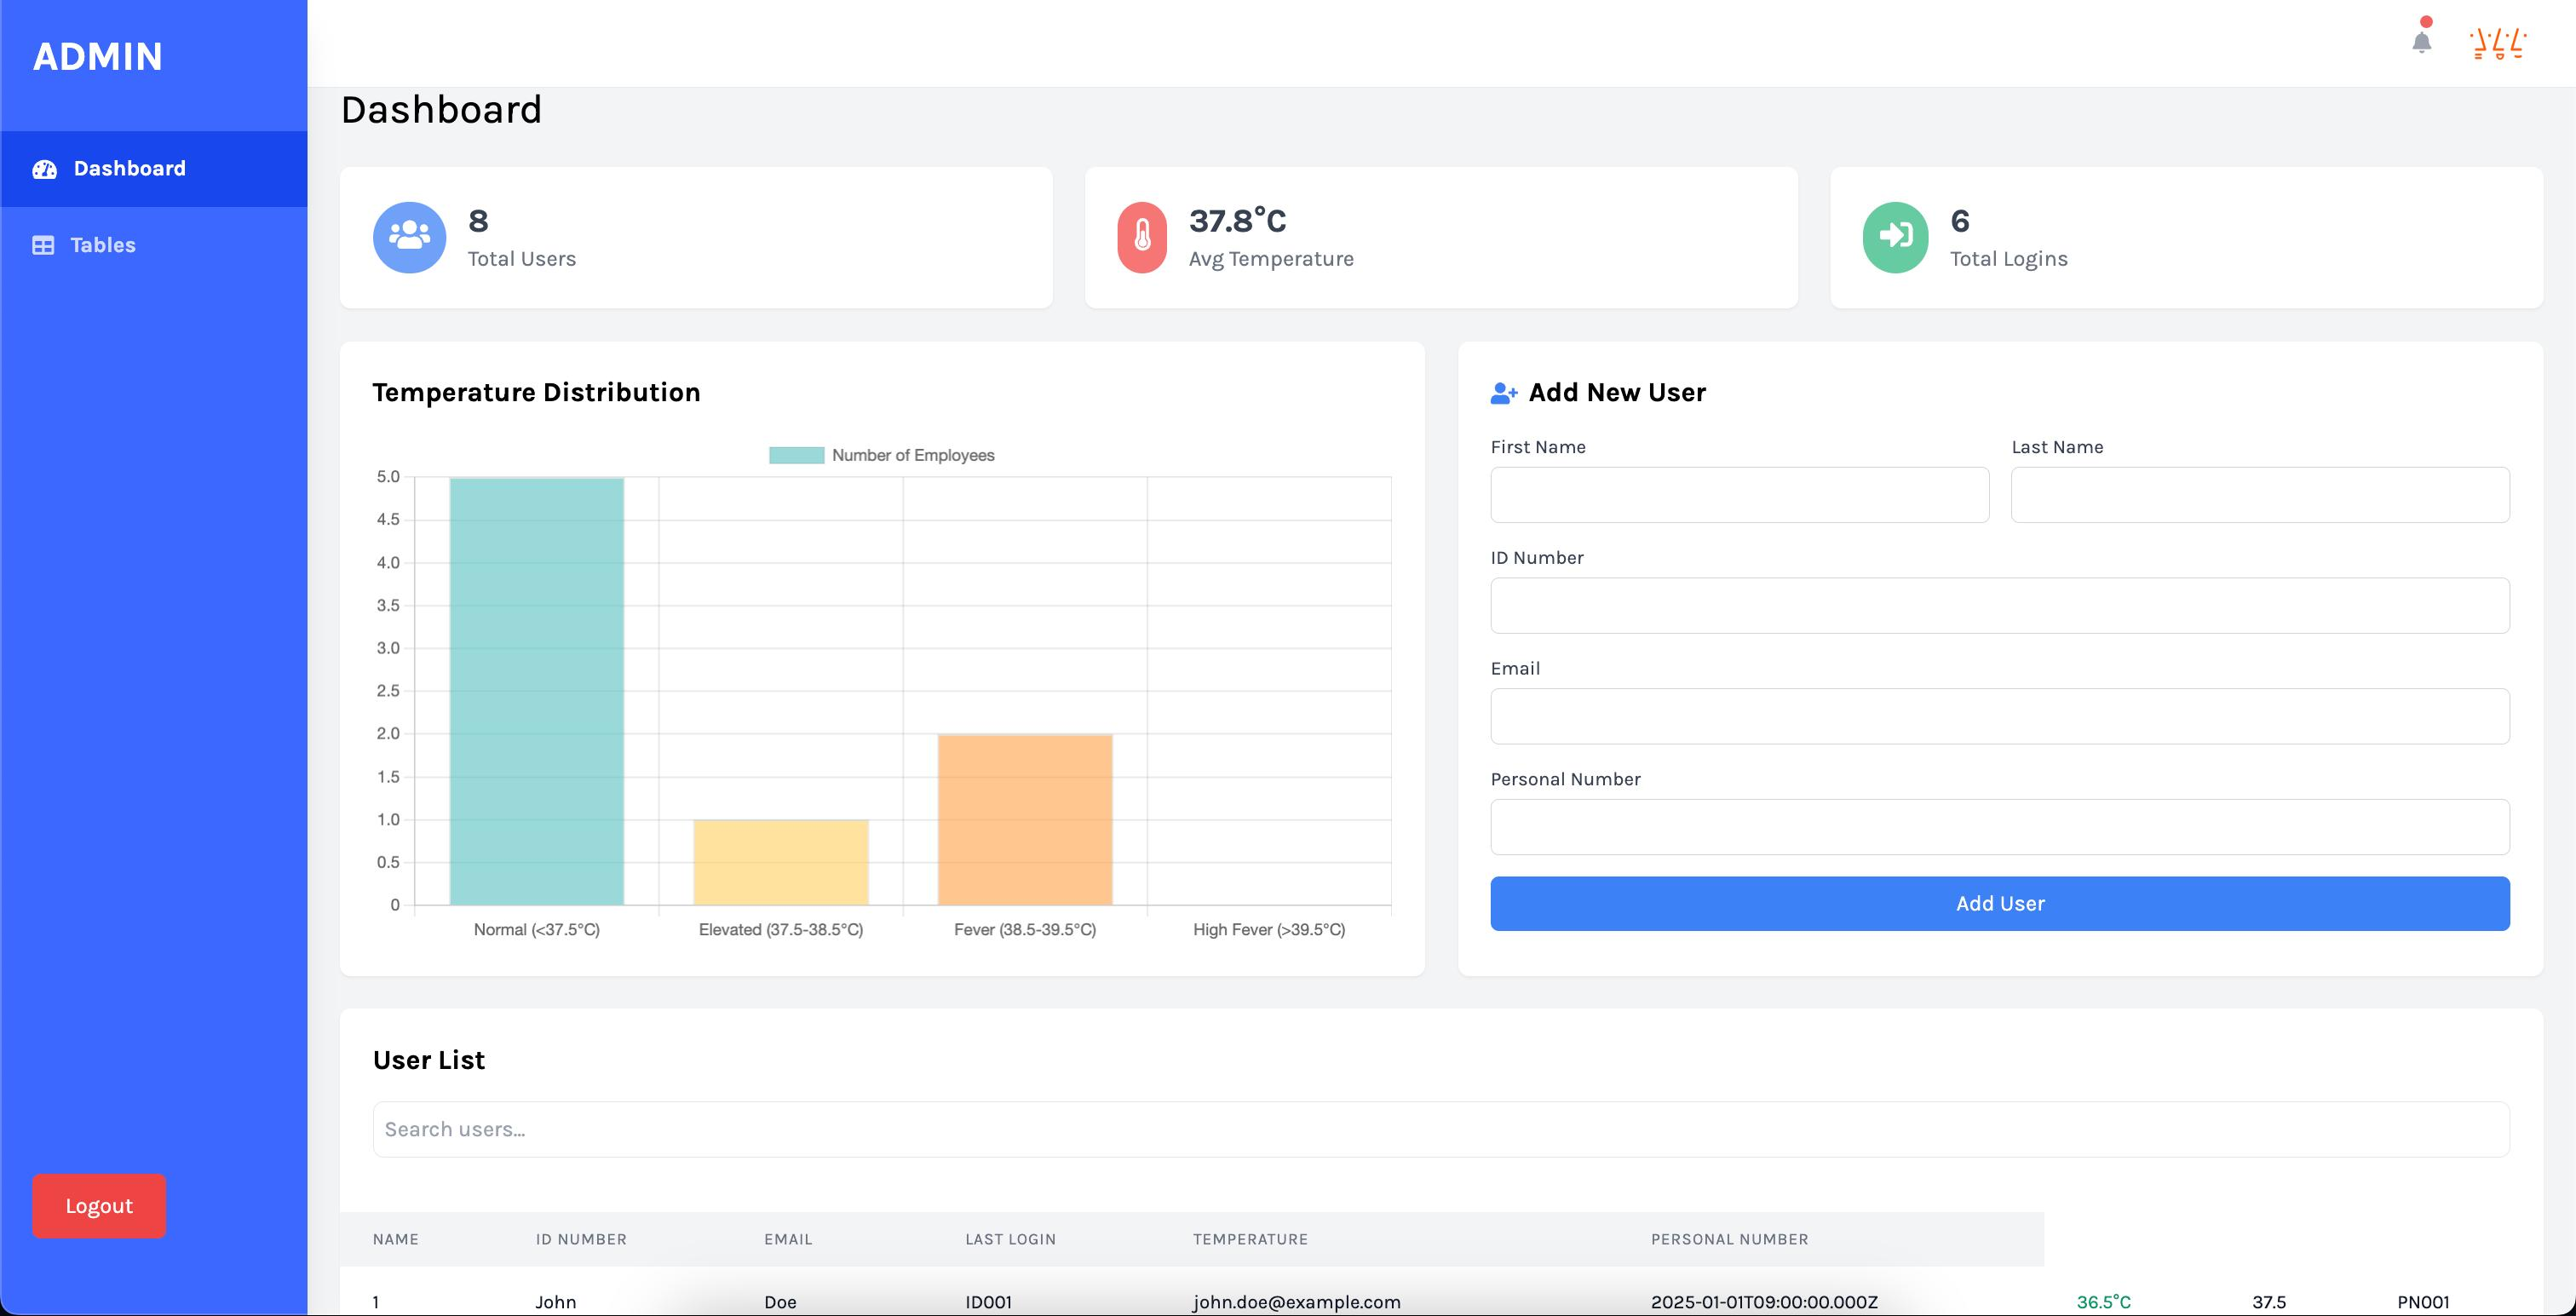
\includegraphics[width=0.4\linewidth]{figures/GUI.jpeg}
	\caption[GUI]{Ausschnitt aus dem Graphical User Interface (GUI)}\label{fig:gui}
\end{figure}
\todo{Bildgröße am Ende anpassen}

Über eine ständig sichtbare Sidebar mit passenden Icons gelangt man schnell zu wichtigen Bereichen wie dem Dashboard oder den Tabellenansichten. Im Dashboard bekommt man einen Überblick über wichtige Kennzahlen – etwa die Anzahl der Nutzer, die Durchschnittstemperatur und die Login-Aktivitäten – die in Echtzeit aktualisiert werden. 

\vspace{1em}
\noindent Neue Benutzer oder Mitarbeiter können über das Login hinzugefügt werden, wobei Eingaben sofort validiert werden und Fehler direkt angezeigt werden. 

\vspace{1em}
\noindent Die Messdaten werden übersichtlich in Diagrammen dargestellt, zum Beispiel zeigt ein Balkendiagramm die Temperaturverteilung und ein anderes Diagramm die Verteilung der Mitarbeiterrollen.

\vspace{1em}
\noindent Zudem sorgen Such- und Filterfunktionen in den Tabellen dafür, dass man die Daten schnell durchsuchen und analysieren kann. Die Anmeldung erfolgt über ein Login-System, das auf JSON Web Tokens (JWT) basiert, sodass nur berechtigte Nutzer Zugriff auf die Anwendung haben.

\vspace{1em}
\noindent\textbf{Fazit:}\newline
Durch die Kombination dieser Technologien entstand eine benutzerfreundliche Webanwendung, die alle wichtigen Daten zentral anzeigt und verwaltet. Die modulare Architektur erlaubt zudem eine einfache Erweiterung, falls zukünftig weitere Anpassungen notwendig werden falls unser Projekt jemals in Produktion gehen würde.


\subsection{API-Dokumentation}
\label{subsec:api-dokumentation}

Die API unterstützt die Benutzer- und Mitarbeiterverwaltung sowie die Kommunikation mit der Datenbank. Im Folgenden sind die wichtigsten Endpunkte und deren Funktion kurz zusammengefasst.


\subsubsection{Allgemeines}

\begin{itemize}
    \item \textbf{Datenformat: }Alle Anfragen und Antworten erfolgen in JSON.
    \item \textbf{Fehler: }Bei ungültigen Anfragen wird eine entsprechende Fehlermeldung mit HTTP-Statuscode zurückgegeben.
    \item \textbf{Port: }Standardmäßig läuft der Server auf Port 3001 (konfigurierbar über .env).
\end{itemize}


\subsubsection{Benutzerverwaltung}

\textbf{Registrierung}
\begin{itemize}
    \item \textbf{Methode: }POST 
    \item \textbf{Endpoint: }/api/register 
    \item \textbf{Body: } \begin{minted}[linenos]{JSON}
{
  "username": "testuser",
  "password": "securepassword"
}
    \end{minted}
    \item \textbf{Antworten: }
    \begin{itemize}
        \item \textit{201 Created: }Benutzer erfolgreich registriert
        \item \textit{400 Bad Request: }Benutzername existiert bereits oder erforderliche Felder fehlen
        \item \textit{500 Internal Server Error: }Fehler beim Speichern in der Datenbank
    \end{itemize}
\end{itemize}
%\todo{Code noch besser formatieren}
\textbf{Login}
\begin{itemize}
    \item \textbf{Methode: }POST 
    \item \textbf{Endpoint: }/api/login  
    \item \textbf{Body: } \begin{minted}[linenos]{JSON}
{
  "username": "testuser",
  "password": "securepassword"
}
    \end{minted}
    \item \textbf{Antworten: }
    \begin{itemize}
        \item \textit{200 OK: }Login erfolgreich, liefert ein JWT-Token (gültig für eine Stunde)
        \item \textit{401 Unauthorized: }Falscher Benutzername oder Passwort
        \item \textit{500 Internal Server Error: }Fehler beim Abrufen des Benutzers
    \end{itemize}
\end{itemize}


\subsubsection{Datenbankverwaltung}

\textbf{Datenbankverbindung testen}
\begin{itemize}
    \item \textbf{Methode: }GET 
    \item \textbf{Endpoint: }/test-db
    \item \textbf{Antworten: }
    \begin{itemize}
        \item \textit{200 OK: }Verbindung erfolgreich
        \item \textit{500 Internal Server Error: }Fehlerhafte Verbindung
    \end{itemize}
\end{itemize}


\subsubsection{Mitarbeiterverwaltung}

\textbf{Mitarbeiter abrufen}
\begin{itemize}
    \item \textbf{Methode: }GET 
    \item \textbf{Endpoint: }/api/employees
    \item \textbf{Antworten: }
    \begin{itemize}
        \item \textit{200 OK: }Array mit allen Mitarbeitern
        \item \textit{500 Internal Server Error: }Fehler beim Abrufen der Daten
    \end{itemize}
\end{itemize}

\textbf{Neuen Mitarbeiter hinzufügen}
\begin{itemize}
    \item \textbf{Methode: }POST 
    \item \textbf{Endpoint: }/api/employess  
    \item \textbf{Body: } \begin{minted}[linenos]{JSON}
{
    "first_name": "Max",
    "last_name": "Mustermann",
    "id_number": "12345",
    "email": "max@example.com",
    "personal_number": "67890"
}
    \end{minted}
    \item \textbf{Antworten: }
    \begin{itemize}
        \item \textit{201 Created: }Mitarbeiter erfolgreich gespeichert
        \item \textit{400 Bad Request: }Fehlende oder ungültige Felder
        \item \textit{500 Internal Server Error: }Fehler beim Speichern des Mitarbeiters
    \end{itemize}
\end{itemize}


\section{Ergebnisse und Diskussion}
\label{sec:ergebnisse_und_diskussion}

\todo[inline, color=green]{Janis}


\section{Fazit und Ausblick}
\label{sec:fazit_und_ausblick}


\subsection{Zusammenfassung der Arbeit}

\todo[inline, color=green]{Janis}


\subsection{Diskussion der Implikationen}

\todo[inline, color=green]{Leopold}
Unsere Untersuchung hat wesentlich dazu beigetragen, grundlegende Zusammenhänge in der Informatik und Elektrotechnik besser zu verstehen. Besonders hervorzuheben ist dabei die Anwendung eines webbasierten Systems welches in Zusammenhang mit einem lokalen Prototyp zusammenspielt. Die PostgreSQL Datenbank könnte durch Zukunftssicherheit auch direkt in Produktion deployt werden. Dasselbe gilt (mit Ausnahme der Authentizität) auch für die Webanwendung.

\vspace{1em}
\noindent Besonders positiv ist, dass die benutzerfreundliche GUI, die auf mobilen Geräten nutzbar ist, zeigt, wie technische Messungen auch für Laien verständlich aufbereitet werden können. Dies fördert nicht nur den Alltagseinsatz neuer Technologien, sondern steigert auch das Bewusstsein für Energieeffizienz und Nachhaltigkeit.

\vspace{1em}
\noindent Insgesamt liefert das Projekt eine fundierte Basis für weiterführende Studien und Anwendungen, die dazu beitragen können, die die Gesundheit und Nachhaltigkeit von Mitarbeitern und Applikationen zu verbessern.


\subsection{Bereiche für zukünftige Arbeiten}

\todo[inline, color=green]{Janis}